\documentclass{scrartcl}
\usepackage{enumitem}
\RequirePackage[utf8]{inputenc}
\RequirePackage[ngerman]{babel}
\RequirePackage[T1]{fontenc}
\RequirePackage{lmodern}
\usepackage{graphicx}
\usepackage{amsmath}


\usepackage{listings}
\usepackage{subfig}
\usepackage{tikz}
\usetikzlibrary{positioning, shapes, snakes, automata}
\usepackage{typearea}
\areaset[5mm]{135mm}{237mm}

\tikzstyle{red} = [color=red, circle, draw]
\tikzstyle{blue} = [color=blue, circle, draw]
\tikzstyle{gray} = [color=gray, circle, draw]
\tikzstyle{green} = [color=green, circle, draw]

\begin{document}

\begin{figure}
\centering
\scalebox{0.8}{
\begin{tikzpicture}[->]
\node[state,initial] (A0) {$A_0$};
\node[state, above right = of A0, yshift=+1.1cm, xshift=0.2cm] (A1) {$A_1$};
\node[state, below right = of A0, yshift=-1.1cm, xshift=0.2cm] (A2) {$A_2$};
\node[state, above right = of A1, yshift=-0.3cm, xshift=0.6cm] (A5) {$A_5$};
\node[state, below right = of A1, yshift=+0.3cm, xshift=0.6cm] (A6) {$A_6$};
\node[state, above right = of A2, yshift=-0.3cm, xshift=0.6cm] (A3) {$A_3$};
\node[state, below right = of A2, yshift=+0.3cm, xshift=0.6cm] (A4) {$A_4$};
\node[state, right = of A6, xshift=0.6cm] (A7) {$A_7$};
\node[state, right = of A3, xshift=0.6cm] (A8) {$A_8$};
\node[state, right = of A0, xshift = 8cm, accepting] (A9) {$A_9$};

\path (A0) edge [bend left] (A1) node[xshift=0.8cm, yshift=1.5cm] {$\tau_{left}$};
\path (A0) edge [bend right] (A2) node[xshift=0.8cm, yshift=-1.5cm] {$\tau_{right}$};

\path (A1) edge [bend left] (A5) node[xshift=1.1cm, yshift=0.9cm] {$\tau_{left}$};
\path (A1) edge [bend right] (A6) node[xshift=1.1cm, yshift=-0.9cm] {$\tau_{right}$};
\path (A2) edge [bend left] (A3) node[xshift=1.1cm, yshift=0.8cm] {$\tau_{right}$};
\path (A2) edge [bend right] (A4) node[xshift=1.1cm, yshift=-0.9cm] {$\tau_{left}$};

\path (A5) edge [bend left] (A9) node[xshift=3.8cm, yshift=-0.9cm] {$\tau_{final}$};
\path (A4) edge [bend right] (A9) node[xshift=3.8cm, yshift=0.8cm] {$\tau_{final}$};

\path (A6) edge (A7) node[xshift=1.3cm, yshift=+0.2cm] {$\tau_{left}$};
\path (A6) edge (A8) node[xshift=1.0cm, yshift=-0.5cm] {$\tau_{right}$};
\path (A3) edge (A7) node[xshift=1.0cm, yshift=+0.5cm] {$\tau_{left}$};
\path (A3) edge (A8) node[xshift=1.3cm, yshift=-0.2cm] {$\tau_{right}$};

\path (A7) edge (A9) node[xshift=1.1cm, yshift=-0.8cm] {$\tau_{final}$};
\path (A8) edge (A9) node[xshift=1.1cm, yshift=+0.8cm] {$\tau_{final}$};
\end{tikzpicture}}
\end{figure}

\begin{figure}
\centering
\begin{tikzpicture}
\coordinate (o) at (0,0) ;
\coordinate (l) at (-6,0); %node[below=0.1cm of l]{-30};
\coordinate (r) at (6,0); %node[below=0.1cm of r]{30};
\coordinate (b) at (0,-3); %node[left=0.1cm of b]{-30};
\coordinate (t) at (0,6); %node[left=0.1cm of t]{30};
\draw (l)--(r) (b)--(t);
% target 1 left ((-10,0),5)
\coordinate (l1) at (-2,0) node[below=0.1cm of l1]{-10};
\fill (l1) circle (2.5pt);
\coordinate (l1a) at (-2,0.8) node[above=0.1cm of l1a, xshift=0.1cm]{5};
\draw (l1) -- (l1a) -- (-1.7,0.8);
\draw (-1.7,0.9) -- (-1.5,0.8) -- (-1.7,0.7) -- cycle;
% target 2 left ((-15,0),8)
\coordinate (l2) at (-3,0) node[below=0.1cm of l2]{-15};
\fill (l2) circle (2.5pt);
\coordinate (l2a) at (-3,0.8) node[above=0.1cm of l2a, xshift=-0.2cm]{7};
\draw (l2) -- (l2a) -- (-3.4,0.8);
\draw (-3.4,0.9) -- (-3.6,0.8) -- (-3.4,0.7) -- cycle;
% target 3 top ((25,1),13)
\coordinate (l3) at (0,4.5) node[left=0.1cm of l3]{25};
\fill (l3) circle (2.5pt);
\coordinate (l3a) at (0.8,4.5) node[right=0.1cm of l3a, yshift=0.4cm]{13};
\draw (l3) -- (l3a) -- (0.8,5.2);
\draw (0.7,5.2) -- (0.8,5.4) -- (0.9,5.2) -- cycle;
\end{tikzpicture}
\caption{Zuvor wäre das Ziel $z=(((-10,0),5))$ im 1D-Fall aus der Liste \emph{Left} eliminiert worden. Mit der zusätzlichen Achse gilt dies nicht mehr für $z$}
\label{fig:BSP}
\end{figure}

\begin{figure}
\centering
\begin{tikzpicture}
\coordinate (a) at (-5,0) node[below=0.1cm of a]{-1000};
\coordinate (b) at (-1,0) node[below=0.1cm of b]{-1};
\coordinate (c) at (0,0) node[below=0.1cm of c]{0};
\coordinate (d) at (1,0) node[below=0.1cm of d]{1};
\coordinate (e) at (5,0) node[below=0.1cm of e]{1000};
\coordinate (f) at (-6,0) node[below=0.1cm of f, xshift=3.0cm]{[...]};
\coordinate (g) at (6,0) node[below=0.1cm of g, xshift=-3.0cm]{[...]};
\fill (a) circle (2.5pt);
\fill (b) circle (2.5pt);
\fill (d) circle (2.5pt);
\fill (e) circle (2.5pt);
\draw (f)--(a)--(b)--(c)--(d)--(e)--(g);
% links 1.
\coordinate (aa) at (-5,0.8);
\draw (a) -- (aa);
\draw (-5,0.8) -- (-5.2,0.8);
\draw (-5.2,0.9) -- (-5.4,0.8) -- (-5.2,0.7) -- cycle;
% links 2.
\coordinate (bb) at (-1,0.8);
\draw (b) -- (bb);
\draw (-1,0.8) -- (-1.7,0.8);
\draw (-1.7,0.9) -- (-1.9,0.8) -- (-1.7,0.7) -- cycle;
% mitte
\draw (0,2) -- (0,1.5) -- (0.4,1.75) -- cycle;
\coordinate (cc) at (0,2);
\draw (c) -- (cc);
% rechts 2.
\coordinate (dd) at (1,0.8);
\draw (d) -- (dd);
\draw (1,0.8) -- (1.7,0.8);
\draw (1.7,0.9) -- (1.9,0.8) -- (1.7,0.7) -- cycle;
% rechts 1.
\coordinate (ee) at (5,0.8);
\draw (e) -- (ee);
\draw (5,0.8) -- (5.2,0.8);
\draw (5.2,0.9) -- (5.4,0.8) -- (5.2,0.7) -- cycle;
\end{tikzpicture}
%\caption{einfaches Gegenspiel}
\label{fig:BSP}
\end{figure}
\newpage
\begin{figure}
\centering
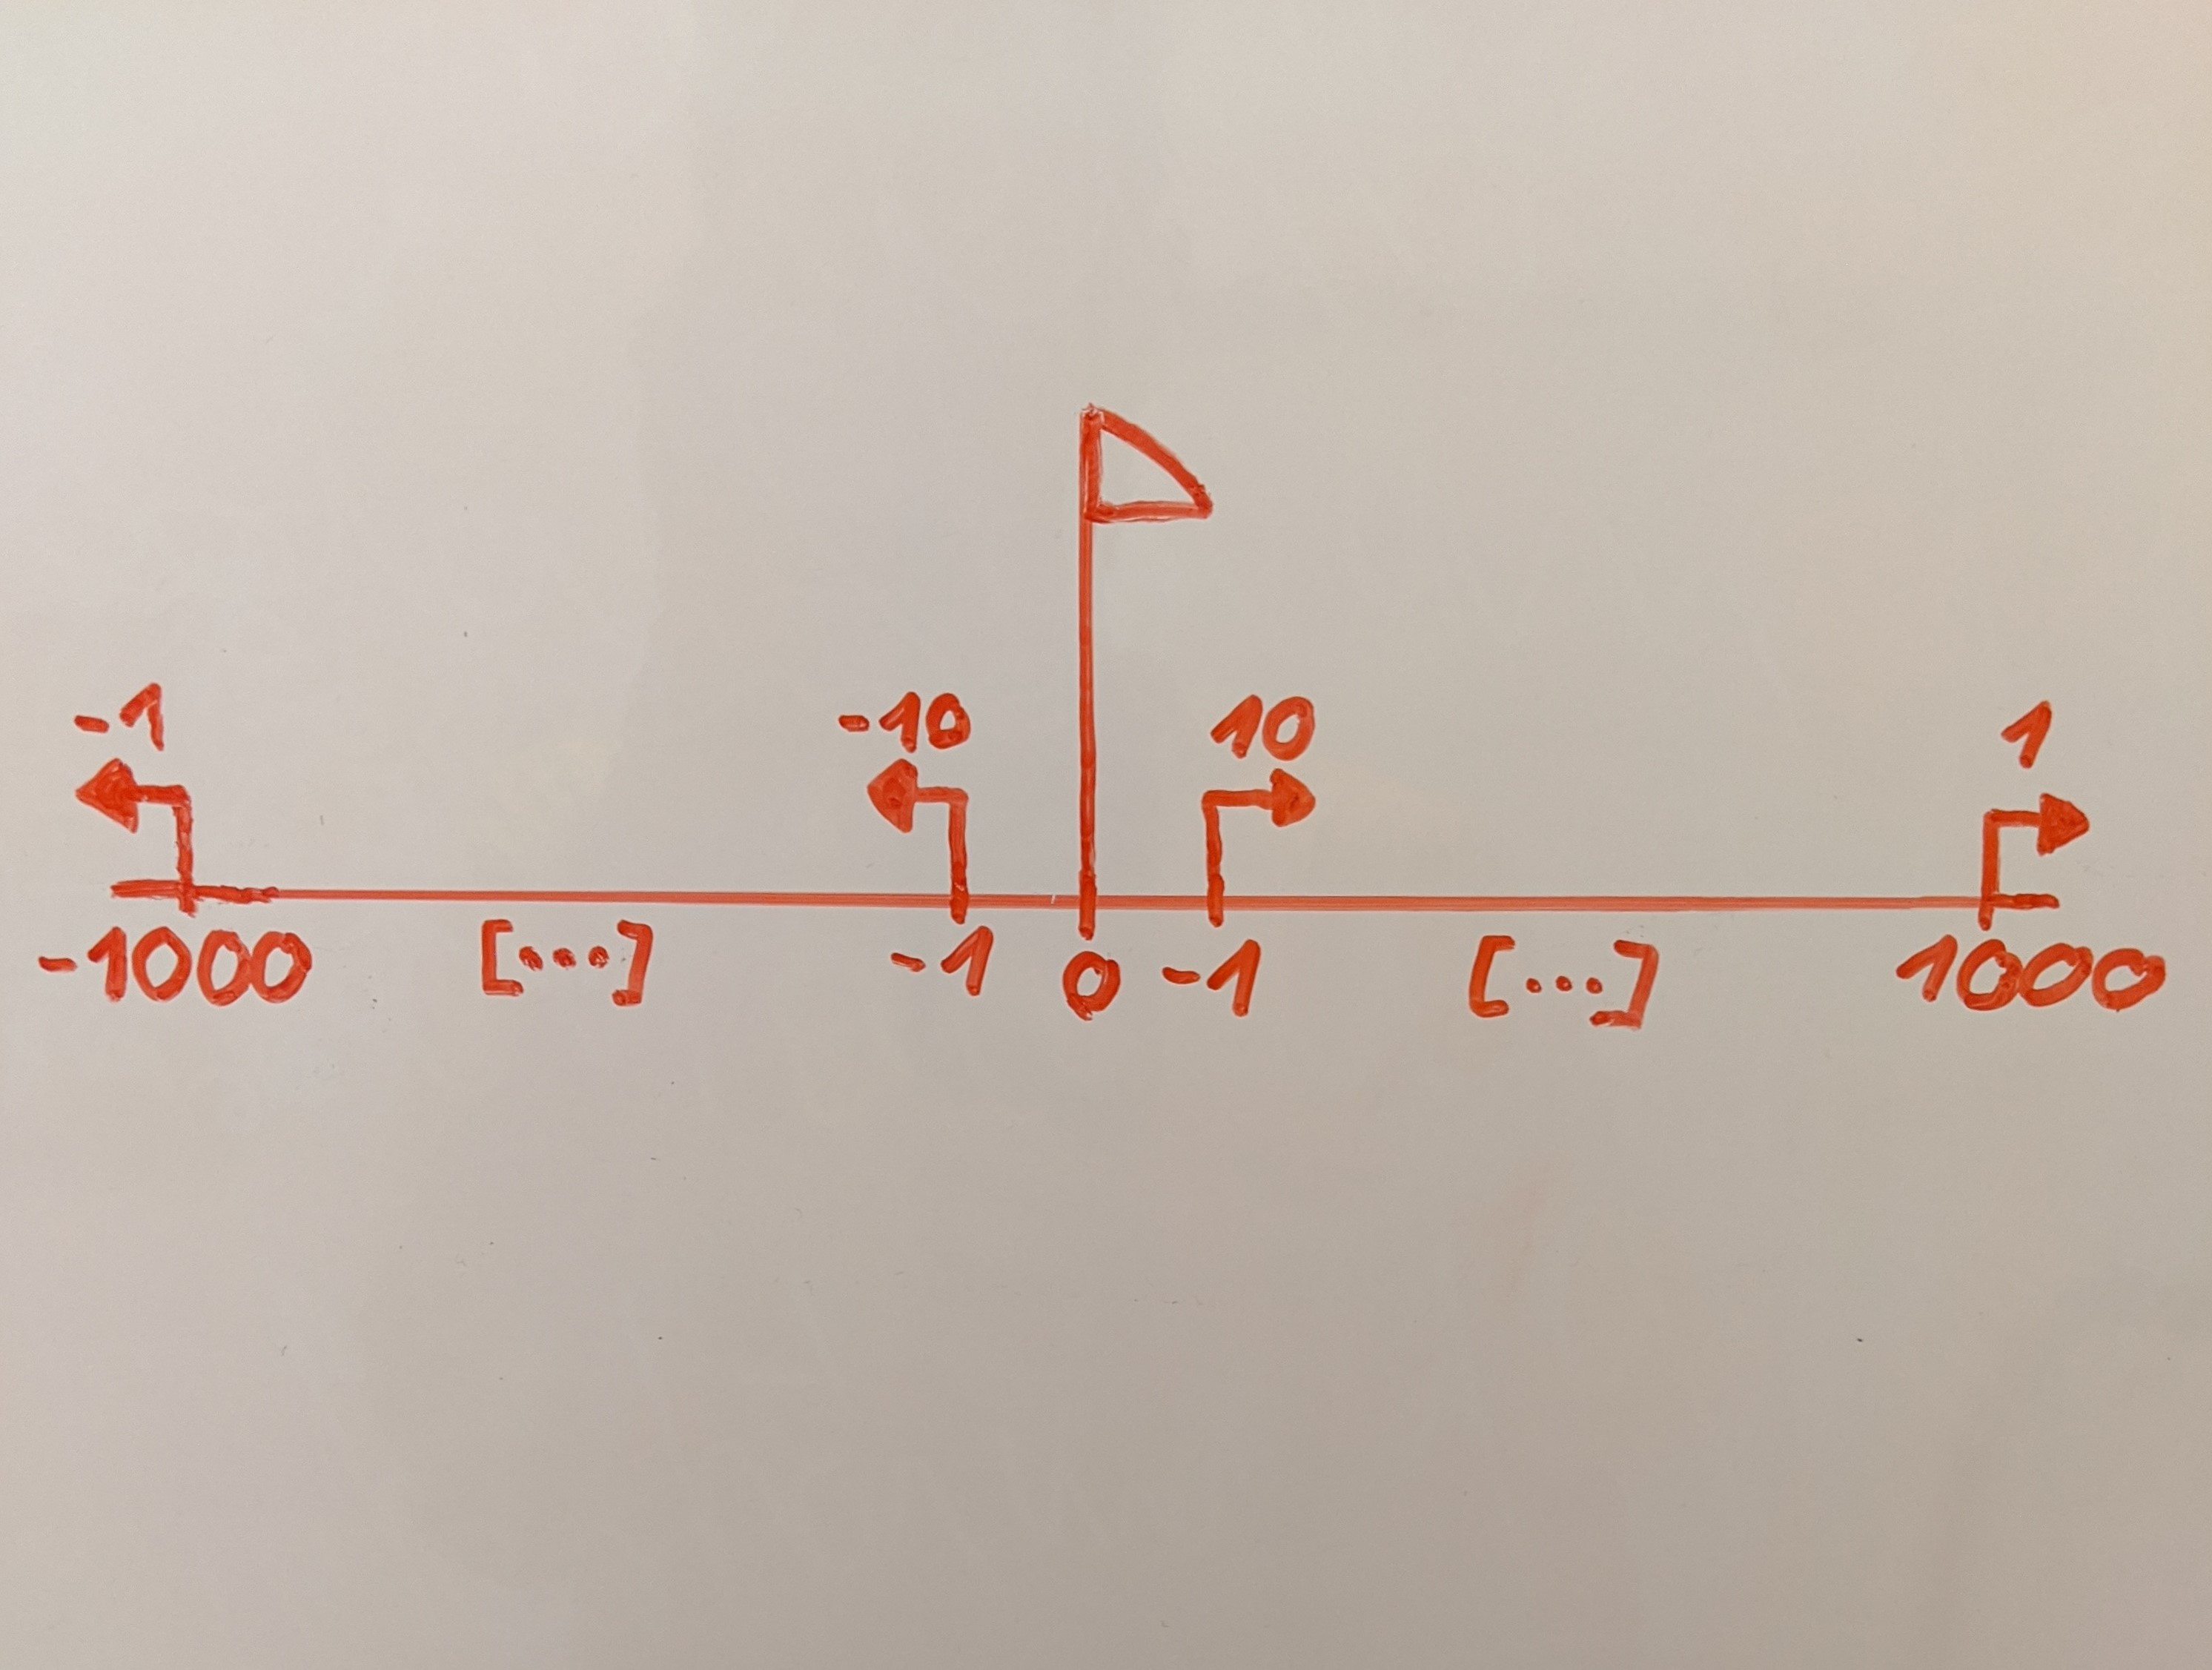
\includegraphics[scale=0.09]{../Grafiken/Whiteboard/GegenBsp1Dim.jpg}
%\caption{einfaches Gegenspiel}
\label{fig:GegenBsp1Dim}
\end{figure}


\begin{tikzpicture}[->,level/.style={sibling distance = 5cm/#1,
  level distance = 1.5cm}]
\node[rectangle, draw, rounded corners=5] (root) {root}
	child { node[red]{$z_1$}
		child { node[blue]{$z_2$}
			child { node[green](1){$z_3$} }
		}
		child { node[green]{$z_3$}
			child { node[blue](2){$z_2$} }
		}
	}
	child { node[blue]{$z_2$}
		child { node[red]{$z_1$}
			child { node[green](3){$z_3$} }
		}
		child { node[green]{$z_3$}
			child { node[red](4){$z_1$} }
		}
	}
	child { node[green]{$z_3$}
		child { node[red]{$z_1$}
			child { node[blue](5){$z_2$} }
		}
		child { node[blue]{$z_2$}
			child { node[red](6){$z_1$} }
		}
	};	
\node[above of=root, yshift=-1cm, xshift=1.5cm] {$\tau_{min} = 6$};
\node[below of=1, yshift=0.35cm] {$\tau_{z_1,z_2,z_3 = 8,5}$};
\node[below of=2, yshift=0.35cm] {$\tau_{z_1,z_3,z_2 = 6}$};
\node[below of=3, yshift=0.35cm] {$\tau_{z_2,z_1,z_3 = 9}$};
\node[below of=4, yshift=0.35cm] {$\tau_{z_2,z_3,z_1 = 12}$};
\node[below of=5, yshift=0.35cm] {$\tau_{z_3,z_1,z_2 = 18}$};
\node[below of=6, yshift=0.35cm] {$\tau_{z_3,z_2,z_1 = 11}$};
\end{tikzpicture}

\begin{tikzpicture}[->,level/.style={sibling distance = 5cm/#1,
  level distance = 1.5cm}]
\node[rectangle, draw, rounded corners=5] (root) {root}
	child { node[red]{$z_1$}
		child { node[blue]{$z_2$}
			child { node[green]{$z_3$} }
		}
		child { node[green]{$z_3$}
			child { node[blue]{$z_2$} }
		}
	}
	child { node[blue]{$z_2$}
		child { node[red]{$z_1$}
			child { node[green]{$z_3$} }
		}
		child { node[green]{$z_3$}
			child { node[red]{$z_1$} }
		}
	}
	child { node[green](z3){$z_3$}
		child { node[gray]{$z_1$}
			child { node[gray]{$z_2$} }
		}
		child { node[gray]{$z_2$}
			child { node[gray]{$z_1$} }
		}
	};	
\node[above of=root, yshift=-1cm, xshift=1.5cm] {$\tau_{min} = 6$};
\node[below of=1, yshift=0.35cm] {$\tau_{z_1,z_2,z_3 = 8,5}$};
\node[below of=2, yshift=0.35cm] {$\tau_{z_1,z_3,z_2 = 6}$};
\node[below of=3, yshift=0.35cm] {$\tau_{z_2,z_1,z_3 = 9}$};
\node[below of=4, yshift=0.35cm] {$\tau_{z_2,z_3,z_1 = 12}$};
\node[right of=z3, xshift=0.2cm] {$\tau_{z_3} = 6.5$};
\node[red, thick, cross out, below, xshift=4.3cm, yshift=-2.1cm, rotate=50] { };
\node[red, thick, cross out, below, xshift=5.7cm, yshift=-2.1cm, rotate=-50] { };
\end{tikzpicture}

\section{Gegenbeispiel Algorithmus von Helvig et. al.}

Dieses Kapitel dient temporär als Gegenbeispiel für den Algorithmus aus \cite{helvig}.
Input: Ziele $Z=\{(-933,13),(-203,-12),(756,8)\}$, Verfolger $\kappa=(0,15)$\\
\textcolor{red}{TODO: Wenn Gegenbsp korrekt, erstelle Grafik}\\
Mit dem Algorithmus von Helvig et. al. würden nun folgende 6 Zustände erstellt werden:
\begin{align*}
&A_0\\
&\{(-203,-12), (756,8)\}\\
&\{(756,8), (-203,-12)\}\\
&\{(-933,13), (756,8)\}\\
&\{(756, 8), (-933,13)\}\\
&A_{final}
\end{align*}
Nun wird durch jeden dieser Zustände in chronologischer Reihenfolge iteriert. Dabei ergeben sich jeweils folgende Zeiten:
\begin{align*}
&\text{Iteration 1:}~t=[0.0, 67.67, 108.0, \infty, \infty, \infty] \\
&\text{Iteration 2:}~t=[0.0, 67.67, 108.0, 548.5, 398.0, \infty] \\
&\text{Iteration 3:}~t=[0.0, 67.67, 108.0, 548.5, 398.0, 2079.33] \\
&\text{Iteration 4:}~t=[0.0, 67.67, 108.0, 548.5, 398.0, 961.67] \\
&\text{Iteration 5:}~t=[0.0, 67.67, 108.0, 548.5, 398.0, 961.67] 
\end{align*}
Bemerke, dass keine Iteration $6$ nötig ist, da nach $A_{final}$ keine Ziele mehr abgefangen werden müssen. Somit hat die vermeintlich optimale Tour eine Dauer von $961,67$-Zeiteinheiten. Dabei werden die Ziele in folgender Reihenfolge abgefangen:
\begin{align*}
&(0,0), ~~~~~ Abfangzeit: 0.0 \\
&(-933, 13), ~Abfangzeit: 33.32 \\
&(-203, -12), Abfangzeit: 67.66 \\
&(756, 8), ~~~Abfangzeit: 398.0 \\
&(0, 0), ~~~~~Abfangzeit: 961.67 
\end{align*}

Wendet man nun den Brute-Force-Algorithmus erhält man folgende Reihenfolge der Ziele:
\begin{align*}
&(0, 0), ~~~~~Abfangzeit: 0.0 \\
&(-933, 13), ~Abfangzeit: 33.32 \\
&(-203, -12), Abfangzeit: 67.66 \\
&(756, 8), ~~~Abfangzeit: 398.0 \\
&(0, 0), ~~~~~Abfangzeit: 660.67 \\
\end{align*}
Zunächst würde man nun davon ausgehen, dass 

\end{document}

%\draw[very thick] (-6,0) -- (6,0);
%\draw (0,0) -- (0,2); 